% Template adapted from the Eurographics SGP 2016 template
\documentclass{6838publ}
\usepackage{6838}
% \input{\string~/.macros}

\SpecialIssuePaper
\electronicVersion 
\ifpdf \usepackage[pdftex]{graphicx} \pdfcompresslevel=9
\else \usepackage[dvips]{graphicx} \fi
\graphicspath{{./assets}}


 
\PrintedOrElectronic

\usepackage{t1enc,dfadobe}
\usepackage{egweblnk}
\usepackage{cite}
\usepackage{lipsum}
\usepackage{amsmath}
\usepackage{amsfonts}
\usepackage{amssymb}


\newcommand{\norm}[1]{\left\lVert#1\right\rVert}
\newcommand\ba{\ensuremath{\mathbf{a}}}
\newcommand\bb{\ensuremath{\mathbf{b}}}
\newcommand\bc{\ensuremath{\mathbf{c}}}
\newcommand\bd{\ensuremath{\mathbf{d}}}
\newcommand\be{\ensuremath{\mathbf{e}}}
\newcommand\bg{\ensuremath{\mathbf{g}}}
\newcommand\bh{\ensuremath{\mathbf{h}}}
\newcommand\bi{\ensuremath{\mathbf{i}}}
\newcommand\bj{\ensuremath{\mathbf{j}}}
\newcommand\bk{\ensuremath{\mathbf{k}}}
\newcommand\bl{\ensuremath{\mathbf{l}}}
\newcommand\bn{\ensuremath{\mathbf{n}}}
\newcommand\bo{\ensuremath{\mathbf{o}}}
\newcommand\bp{\ensuremath{\mathbf{p}}}
\newcommand\bq{\ensuremath{\mathbf{q}}}
\newcommand\br{\ensuremath{\mathbf{r}}}
\newcommand\bs{\ensuremath{\mathbf{s}}}
\newcommand\bt{\ensuremath{\mathbf{t}}}
\newcommand\bu{\ensuremath{\mathbf{u}}}
\newcommand\bv{\ensuremath{\mathbf{v}}}
\newcommand\bw{\ensuremath{\mathbf{w}}}
\newcommand\bx{\ensuremath{\mathbf{x}}}
\newcommand\by{\ensuremath{\mathbf{y}}}
\newcommand\bz{\ensuremath{\mathbf{z}}}
\newcommand\bA{\ensuremath{\mathbf{A}}}
\newcommand\bB{\ensuremath{\mathbf{B}}}
\newcommand\bC{\ensuremath{\mathbf{C}}}
\newcommand\bD{\ensuremath{\mathbf{D}}}
\newcommand\bE{\ensuremath{\mathbf{E}}}
\newcommand\bF{\ensuremath{\mathbf{F}}}
\newcommand\bG{\ensuremath{\mathbf{G}}}
\newcommand\bH{\ensuremath{\mathbf{H}}}
\newcommand\bI{\ensuremath{\mathbf{I}}}
\newcommand\bJ{\ensuremath{\mathbf{J}}}
\newcommand\bK{\ensuremath{\mathbf{K}}}
\newcommand\bL{\ensuremath{\mathbf{L}}}
\newcommand\bM{\ensuremath{\mathbf{M}}}
\newcommand\bN{\ensuremath{\mathbf{N}}}
\newcommand\bO{\ensuremath{\mathbf{O}}}
\newcommand\bP{\ensuremath{\mathbf{P}}}
\newcommand\bQ{\ensuremath{\mathbf{Q}}}
\newcommand\bR{\ensuremath{\mathbf{R}}}
\newcommand\bS{\ensuremath{\mathbf{S}}}
\newcommand\bT{\ensuremath{\mathbf{T}}}
\newcommand\bU{\ensuremath{\mathbf{U}}}
\newcommand\bV{\ensuremath{\mathbf{V}}}
\newcommand\bW{\ensuremath{\mathbf{W}}}
\newcommand\bX{\ensuremath{\mathbf{X}}}
\newcommand\bY{\ensuremath{\mathbf{Y}}}
\newcommand\bZ{\ensuremath{\mathbf{Z}}}
\newcommand\Ba{\ensuremath{\mathbb{a}}}
\newcommand\Bb{\ensuremath{\mathbb{b}}}
\newcommand\Bc{\ensuremath{\mathbb{c}}}
\newcommand\Bd{\ensuremath{\mathbb{d}}}
\newcommand\Be{\ensuremath{\mathbb{e}}}
\newcommand\Bf{\ensuremath{\mathbb{f}}}
\newcommand\Bg{\ensuremath{\mathbb{g}}}
\newcommand\Bh{\ensuremath{\mathbb{h}}}
\newcommand\Bi{\ensuremath{\mathbb{i}}}
\newcommand\Bj{\ensuremath{\mathbb{j}}}
\newcommand\Bk{\ensuremath{\mathbb{k}}}
\newcommand\Bl{\ensuremath{\mathbb{l}}}
\newcommand\Bm{\ensuremath{\mathbb{m}}}
\newcommand\Bn{\ensuremath{\mathbb{n}}}
\newcommand\Bo{\ensuremath{\mathbb{o}}}
\newcommand\Bp{\ensuremath{\mathbb{p}}}
\newcommand\Bq{\ensuremath{\mathbb{q}}}
\newcommand\Br{\ensuremath{\mathbb{r}}}
\newcommand\Bs{\ensuremath{\mathbb{s}}}
\newcommand\Bt{\ensuremath{\mathbb{t}}}
\newcommand\Bu{\ensuremath{\mathbb{u}}}
\newcommand\Bv{\ensuremath{\mathbb{v}}}
\newcommand\Bw{\ensuremath{\mathbb{w}}}
\newcommand\Bx{\ensuremath{\mathbb{x}}}
\newcommand\By{\ensuremath{\mathbb{y}}}
\newcommand\Bz{\ensuremath{\mathbb{z}}}
\newcommand\BA{\ensuremath{\mathbb{A}}}
\newcommand\BB{\ensuremath{\mathbb{B}}}
\newcommand\BC{\ensuremath{\mathbb{C}}}
\newcommand\BD{\ensuremath{\mathbb{D}}}
\newcommand\BE{\ensuremath{\mathbb{E}}}
\newcommand\BF{\ensuremath{\mathbb{F}}}
\newcommand\BG{\ensuremath{\mathbb{G}}}
\newcommand\BH{\ensuremath{\mathbb{H}}}
\newcommand\BI{\ensuremath{\mathbb{I}}}
\newcommand\BJ{\ensuremath{\mathbb{J}}}
\newcommand\BK{\ensuremath{\mathbb{K}}}
\newcommand\BL{\ensuremath{\mathbb{L}}}
\newcommand\BM{\ensuremath{\mathbb{M}}}
\newcommand\BN{\ensuremath{\mathbb{N}}}
\newcommand\BO{\ensuremath{\mathbb{O}}}
\newcommand\BP{\ensuremath{\mathbb{P}}}
\newcommand\BQ{\ensuremath{\mathbb{Q}}}
\newcommand\BR{\ensuremath{\mathbb{R}}}
\newcommand\BS{\ensuremath{\mathbb{S}}}
\newcommand\BT{\ensuremath{\mathbb{T}}}
\newcommand\BU{\ensuremath{\mathbb{U}}}
\newcommand\BV{\ensuremath{\mathbb{V}}}
\newcommand\BW{\ensuremath{\mathbb{W}}}
\newcommand\BX{\ensuremath{\mathbb{X}}}
\newcommand\BY{\ensuremath{\mathbb{Y}}}
\newcommand\BZ{\ensuremath{\mathbb{Z}}}
\newcommand\balpha{\ensuremath{\mbox{\boldmath$\alpha$}}}
\newcommand\bbeta{\ensuremath{\mbox{\boldmath$\beta$}}}
\newcommand\btheta{\ensuremath{\mbox{\boldmath$\theta$}}}
\newcommand\bphi{\ensuremath{\mbox{\boldmath$\phi$}}}
\newcommand\bpi{\ensuremath{\mbox{\boldmath$\pi$}}}
\newcommand\bpsi{\ensuremath{\mbox{\boldmath$\psi$}}}
\newcommand\bmu{\ensuremath{\mbox{\boldmath$\mu$}}}

\newcommand\R{\ensuremath{\mathbb{R}}} % Real numbers
\newcommand\Z{\ensuremath{\mathbb{Z}}} % Integers


\DeclareMathOperator*{\diag}{diag} % Diagonal matrix
\newcommand\p[1]{\ensuremath{\left( #1 \right)}} % Parenthesis ()
\newcommand\pa[1]{\ensuremath{\left\langle #1 \right\rangle}} % <>
\newcommand\pb[1]{\ensuremath{\left[ #1 \right]}} % []
\newcommand\pc[1]{\ensuremath{\left\{ #1 \right\}}} % {}


\title[]{Probabilistic Optimal Transport based Diffeomorphic Registration}

\author[P.W.]
       {Peiqi Wang
        \\
        MIT Department of Electrical Engineering and Computer Science\\
       }

\begin{document}

\teaser{
 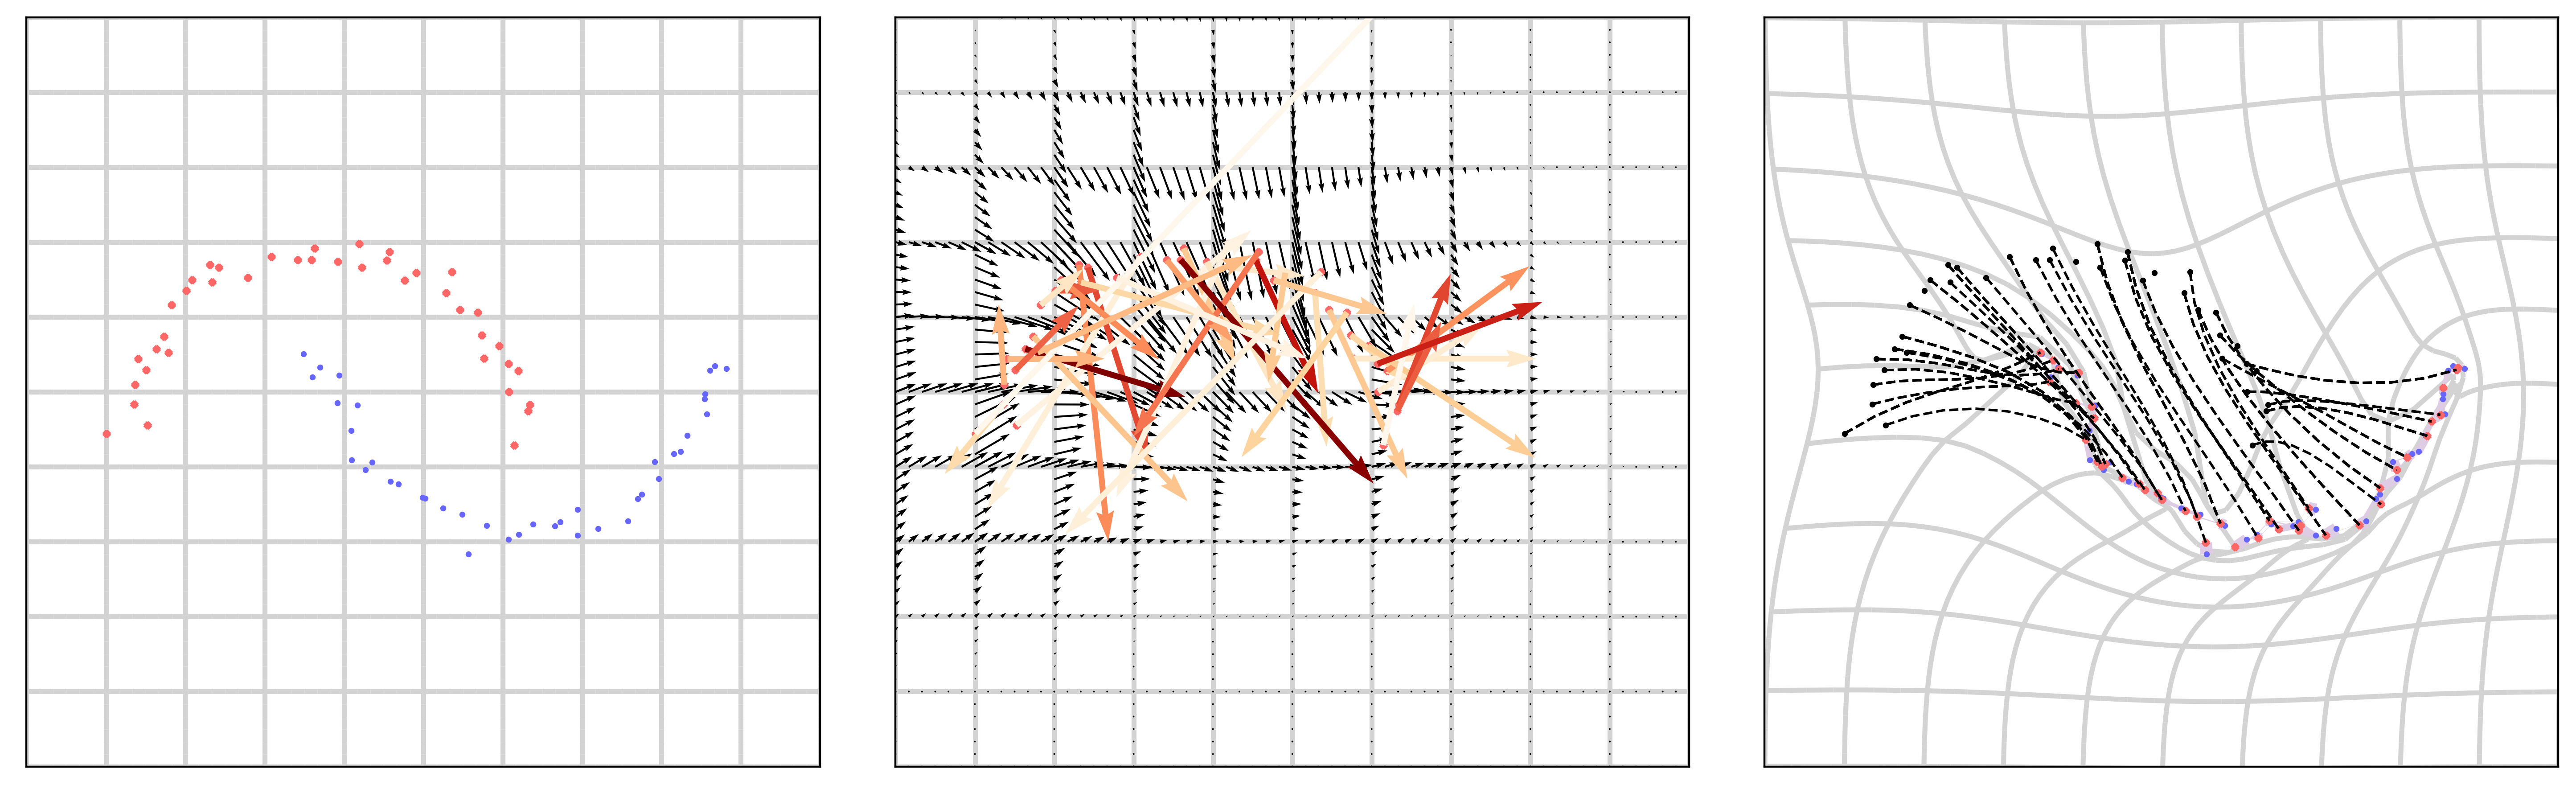
\includegraphics[width=.9\linewidth]{{assets/amoeba/plt_lddmm_points}}
 \centering
  \caption{The red bat is registered to blue amoeba, showing uncertainty of the transformation}
\label{fig:teaser}
}

\maketitle

\begin{abstract}

\end{abstract}

\section{Introduction}

 
% narrow in no topic: remind this is a graphics paper, need to help them to figure out what topic and area of research. no need to wax poetic about topic's importance


% dig a hole: convince reader there is a problem with the state of the world. prior work may exist but its missing something important or there is a missing opportunity. the reading should be drooling for a bright future just out of reach

Diffeomorphic registration of shapes with unknown correspondence is an important step in medical data processing. The choice of similarity measure for correct matching distinguishes the different algorithms in this domain. Recent work explored the use of optimal transport distance as a global measure of similarity between discrete representation of shapes \cite{feydyOptimalTransportDiffeomorphic2017a,feydyFastScalableOptimal2019}. However, a point estimate of the transformation can generate errors left un-noticed by downstream processing pipelines. In addition, the solution is sensitive to hyperparameters of the model, requiring manual tuning for each new shape. Furthermore, the algorithm scales poorly due to the need to generate valid diffeomorphic transformations as well as to solve an optimal transport problem at each iteration.

% fill the hole: to show reader how/why the paper will fix these problems and deliver us into a better place. don't need a whirlwind summary of technical details, but need reader's convinced to keep reading. 

We propose to extend optimal transport based diffeomorphic registration to probabilistic setting. Our method interprets the diffeomorphic transformation as a random variable, and estimates its parameters using variational inference. Naturally, the probabilistic formulation provides us with uncertainty estimates of both the transformation as well as the uncertainty of its effect on shapes. Hyperparameters such as the degree of smoothness of the transformation parameterizes the variational distribution, and thus can be optimized. In addition, we explored links to interdomain inducing variables as a way to reduce computation needed to generate valid diffeomorphic transformations \cite{figueiras-vidalInterdomainGaussianProcesses2009a}.


\section{Related Work}

% Descriptions of and citations to academic research papers and/or existing software products related to your work.  Here is an example of how to cite a paper~\cite{solomon-2016}; see \texttt{6838bibsample.bib} for bibliography entries.


\section{Technical Approach}\label{sec:technical_approach}


\subsection{Diffeomorphic Registration}


\section{Diffeomorphic Registration}




\cite{begComputingLargeDeformation2005} 


proposes lddmm for registering images. The goal of the paper is to register two images $I_0,I_1: \Omega\to\R^d$ where $\Omega\subset\R^n$ (n=2 for 2d images) by computing a diffeomorphic coordinate transformation $\varphi:\Omega\to\Omega$ such that the pullback of $I_0$ by $\varphi^{01}$, i.e. $\varphi.I_0 = I\circ \varphi^{-1}$, is registered to the target image $I_1$. Previous work on non-rigid registration approximates $\varphi$ as locally linear, e.g. $\varphi(x) = x + u(x)$ for some displacement vector field $u:\Omega\to\R^n$; However, this assumption breaks down when there is large displacement of objects within the two images. Instead of solving for the transformation directly, the paper proposes to solve for a time-varying velocity vector field $v_t: \Omega\to\R^n$ for $t\in [0,1]$ that dictates dynamics of time-varying transformations $\phi_t: \Omega\to\Omega$, $\frac{d}{dt} \phi_t = v_t(\phi_t) \quad \phi_0 = \text{Id}$ and that the desired transformation $\varphi$ is the endpoint of the above ODE problem, $\varphi  = \phi_1 = \phi_0 + \int_0^1 v_t(\phi_t) \, dt$.
It has been shown that if the velocity vectors are sufficiently smooth, then $\varphi$ is a diffeomorphic map. Let $V$ be the space of velocity fields with norm $\norm{f}_V = \norm{Lf}_{L^2}$ for $L = (-\alpha \nabla^2 + \gamma)^{\beta} I$, we are interested to find velocity fields that are smooth and that the resulting pullback image is similar to the target image, captured by the follwing energy functional.

\begin{align}
    E(v)
        = \int_0^1 \norm{v_t}_V^2 \, dt + \frac{1}{\sigma^2} \norm{ I_0 \circ \phi_1^{-1} - I_1 }_{L^2}^2
\end{align}
where $v := \pc{v_t}$ satisfies $\dot{\phi_t} =  v_t(\phi_t)$. The velocity fields $v_t$ can be optimized using gradient descent. Once an estimate of velocity field is estimated $\hat{v}$, the resulting transformation $\hat{\varphi}$ can be computed via numerical integration of the ODE system. Of particular interest to this method is that the optimization can be interpreted as finding the (discretized) geodesic path on manifold of diffeomorphisms connecting $I_0,I_1$, and that the length of geodesic $\int_0^1 \norm{v_t}_V \, dt$ is a metric distance between images connected via the diffeomorphism at the end point of the flow.



% \section{Geodesic Shooting}

% \cite{millerGeodesicShootingComputational2006,vialardDiffeomorphic3DImage2012} are good references for geodesic shooting of point set and images, albeit hard to understand. \cite{joshiLandmarkMatchingLarge2000} proposed large deformation registration for landmarks, \cite{vaillantStatisticsDiffeomorphismsTangent2004,allassonniereGeodesicShootingDiffeomorphic2005} proposed to flow shape along its geodesics using initial momentum for registering landmarks and textured mesh respectively; both are more accessible introduction to geodesic shooting for point set. Jean Feydy's phd thesis is also pretty helpful and gives good intuition \cite{feydyGeometricDataAnalysis2020}.

% Instead of integrating a time-varying velocity fields to get a diffeomorphic transformation, geodesic shooting evolves the shape from initial momentum. Let $\Omega \subset\R^D$ be ambient space. Let the space of smooth velocity fields $V$ as a rkhs over $\Omega$ characterized by kernel $k:\Omega\times\Omega\to\R^{D\times D}$ satisfying vector-valued reproducing property $\inner{k(x,\cdot)y}{v}_{V} = \inner{v(x)}{y}_{\R^D}$ for all $y\in\R^D, v\in V$. For landmarks, we assume we are trying to seek time-varying velocity field $v_t\in V$ matching template $(x^1,\cdots,x^n)\subset \Omega^N$ and target $(y^1,\cdots,y^n)\subset\Omega^N$ points.
% \begin{align}
%     \min_{v_t:t\in [0,1]} \,
%         &\frac{1}{2} \int_0^1 \norm{v_t}_V^2 \, dt + \frac{1}{2\sigma^2} \sum_{i=1}^N \norm{\varphi(x^i) - y^i}_{\R^{D}}^2 \\
%         \text{where}
%             &\quad \varphi = \phi_1 = x + \int_0^1 v_t(\phi_t(x)) \, dt \\
%             &\quad \frac{d}{dt}\phi_t(x) = v_t(\phi_t(x)) \quad\quad \phi_0 = \text{Id}
% \end{align}
% For $\int_0^1 \norm{v_t}_V \, dt < \infty$, $\varphi$ is a diffeomorphism. Let $q_t^i = \phi_t(x^i) \in \R^D$ be application of transformation $\phi_t$ to point $x^i$. Denote $q_t = (q_t^1, \cdots, q_t^N) \in \R^{ND}$ as action of $\phi_t$ to a set of points and $K(q_t,q_t) \in \R^{ND\times ND}$ be kernel matrix for velocity vector field at $q_t$ consisting of $N\times N$ blocks of $K(q^i,q^j) \in \R^{D\times D}$. \cite{joshiLandmarkMatchingLarge2000} argues for a Lagrangian view of previous Eulerian problem. Instead of solving for flow velocity $v(x,t)$ for all $x\in\Omega, t\in [0,1]$, it suffices to solve for the flow velocity $\dot{q}_t$ of particles,
% \begin{align}
%     \min_{\dot{q}_t:t\in [0,1]}
%         &\frac{1}{2} \int_0^1 \inner{\dot{q}_t}{K(q_t,q_t)^{-1}\dot{q}_t} \, dt + \frac{1}{2\sigma^2} \norm{q_1 - y}_{\R^{ND}}^2
% \end{align}
% and that the resulting flow velocity in the Eulerian coordinates $\Omega$ can be interpolated from $\dot{q}_t$,
% \begin{align}
%     v_t(x)
%         = K(x, q_t) p_t
%     \quad\quad
%     p_t
%         = K(q_t, q_t)^{-1} \dot{q}_t
% \end{align}
% where $p_t^i \in \R^{D}$ is the momenta associated with point $q_t^i$. As a side note, this interpolation is akin to computing posterior mean of a gaussian process regression of velocity fields, i.e. $v_t(x) = K(x,q_t) K(q_t,q_t)^{-1} \dot{q}_t$. Note the integrand of rkhs norm can be viewed as Lagrangian of of a system of ND particles. \cite{millerGeodesicShootingComputational2006} argues the dynamics of these particles in canonical coordinates $(q_t,p_t)$ follows the Geodesic equations with initial condition $q_0 = x, p_0$,
% \begin{align}
%     \dot{q}_t
%         = \frac{\partial \sH(q_t,p_t)}{\partial p}
%     \quad\quad
%     \dot{p}_t
%         = - \frac{\partial \sH(q_t,p_t)}{\partial q}
%     \label{eq:geodesic_equations}
% \end{align}
% and that the Hamiltonian $\sH(q_t,p_t) = \frac{1}{2}\inner{p_t}{K(q_t,q_t)p_t} = \frac{1}{2}\inner{K(q_t,q_t)^{-1}\dot{q}_t}{\dot{q}_t}$ is preseved by the flow, $\sH(q_0,p_0)  = \sH(q_t,p_t)$ for all $t\in [0,1]$ and therefore, $\int_0^1 \sH(q_t,p_t) \, dt = \sH(q_0, p_0) = \frac{1}{2} \inner{ p_0 }{ K(q_0,q_0) p_0 }$. We arrive at a registration problem where we optimize over the initial or \textit{shooting momentum} $p_0$ so that $q_1 := q_1(x,p_0)$ is close in some sense to target $y$,
% \begin{align}
%     \min_{p_0\in\R^{ND}} \,
%         \frac{1}{2} \inner{ p_0 }{ K(x,x) p_0 } + \frac{1}{2\sigma^2} \norm{q_1 - y}_{\R^{ND}}^2
%     \label{eq:optimization_momentum_landmark}
% \end{align}
% Optimization involves a forward integration of $(q_t,p_t)$ via (\ref{eq:geodesic_equations}) to get transformed particles $q_1$, compute the gradient of objective (\ref{eq:optimization_momentum_landmark}) with respect to initial momentum, and do gradient update iteratively.


% \begin{center} 
% \begin{figure}[h!]
%     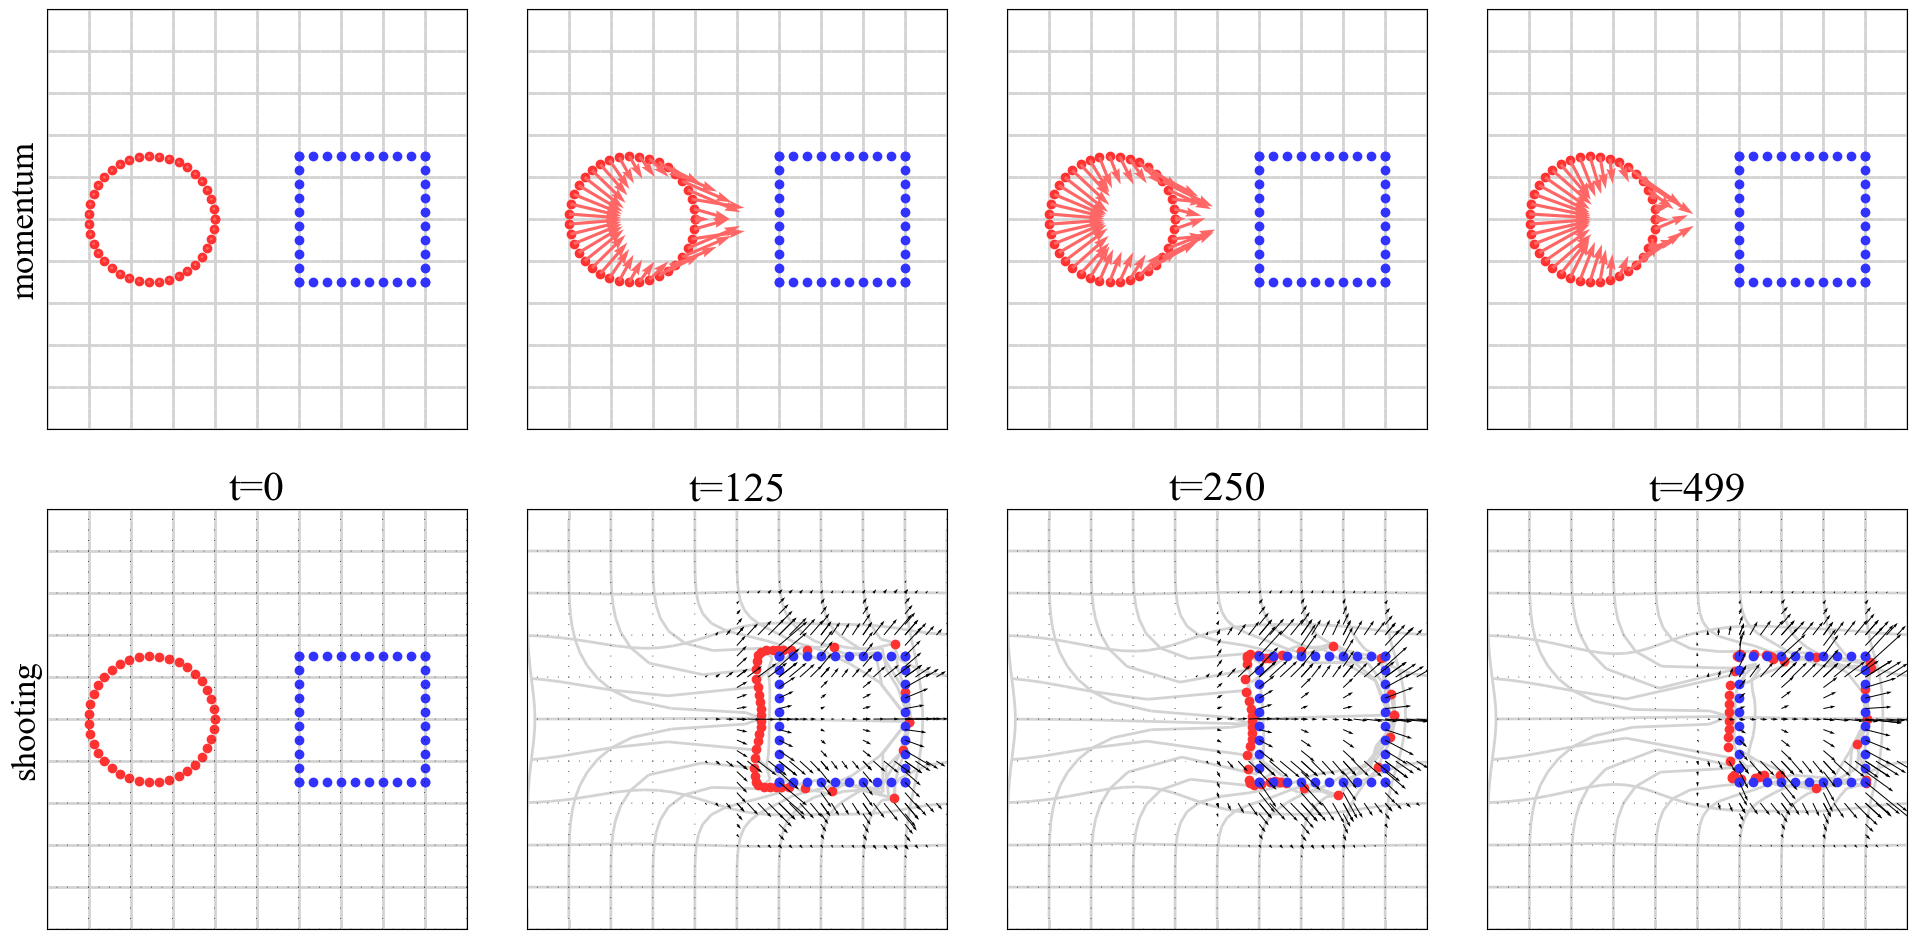
\includegraphics[width=\textwidth]{assets/plt_shooting} 
%     \caption{Geodesic shooting with an Euler integrator with time step of $\delta t = .1$. The velocity field is represented using a radial basis kernel with $\sigma=.25$. We show trajectory of $q_t$ (red dots) with momentum $p_t$ (blue arrow) and interpolated velocity fields at grid points (black). We see Hamiltonian is approximately conserved!}
%     \label{fig:plt_shooting}
% \end{figure} 
% \end{center} 


% \begin{center} 
% \begin{figure}[h!]
%     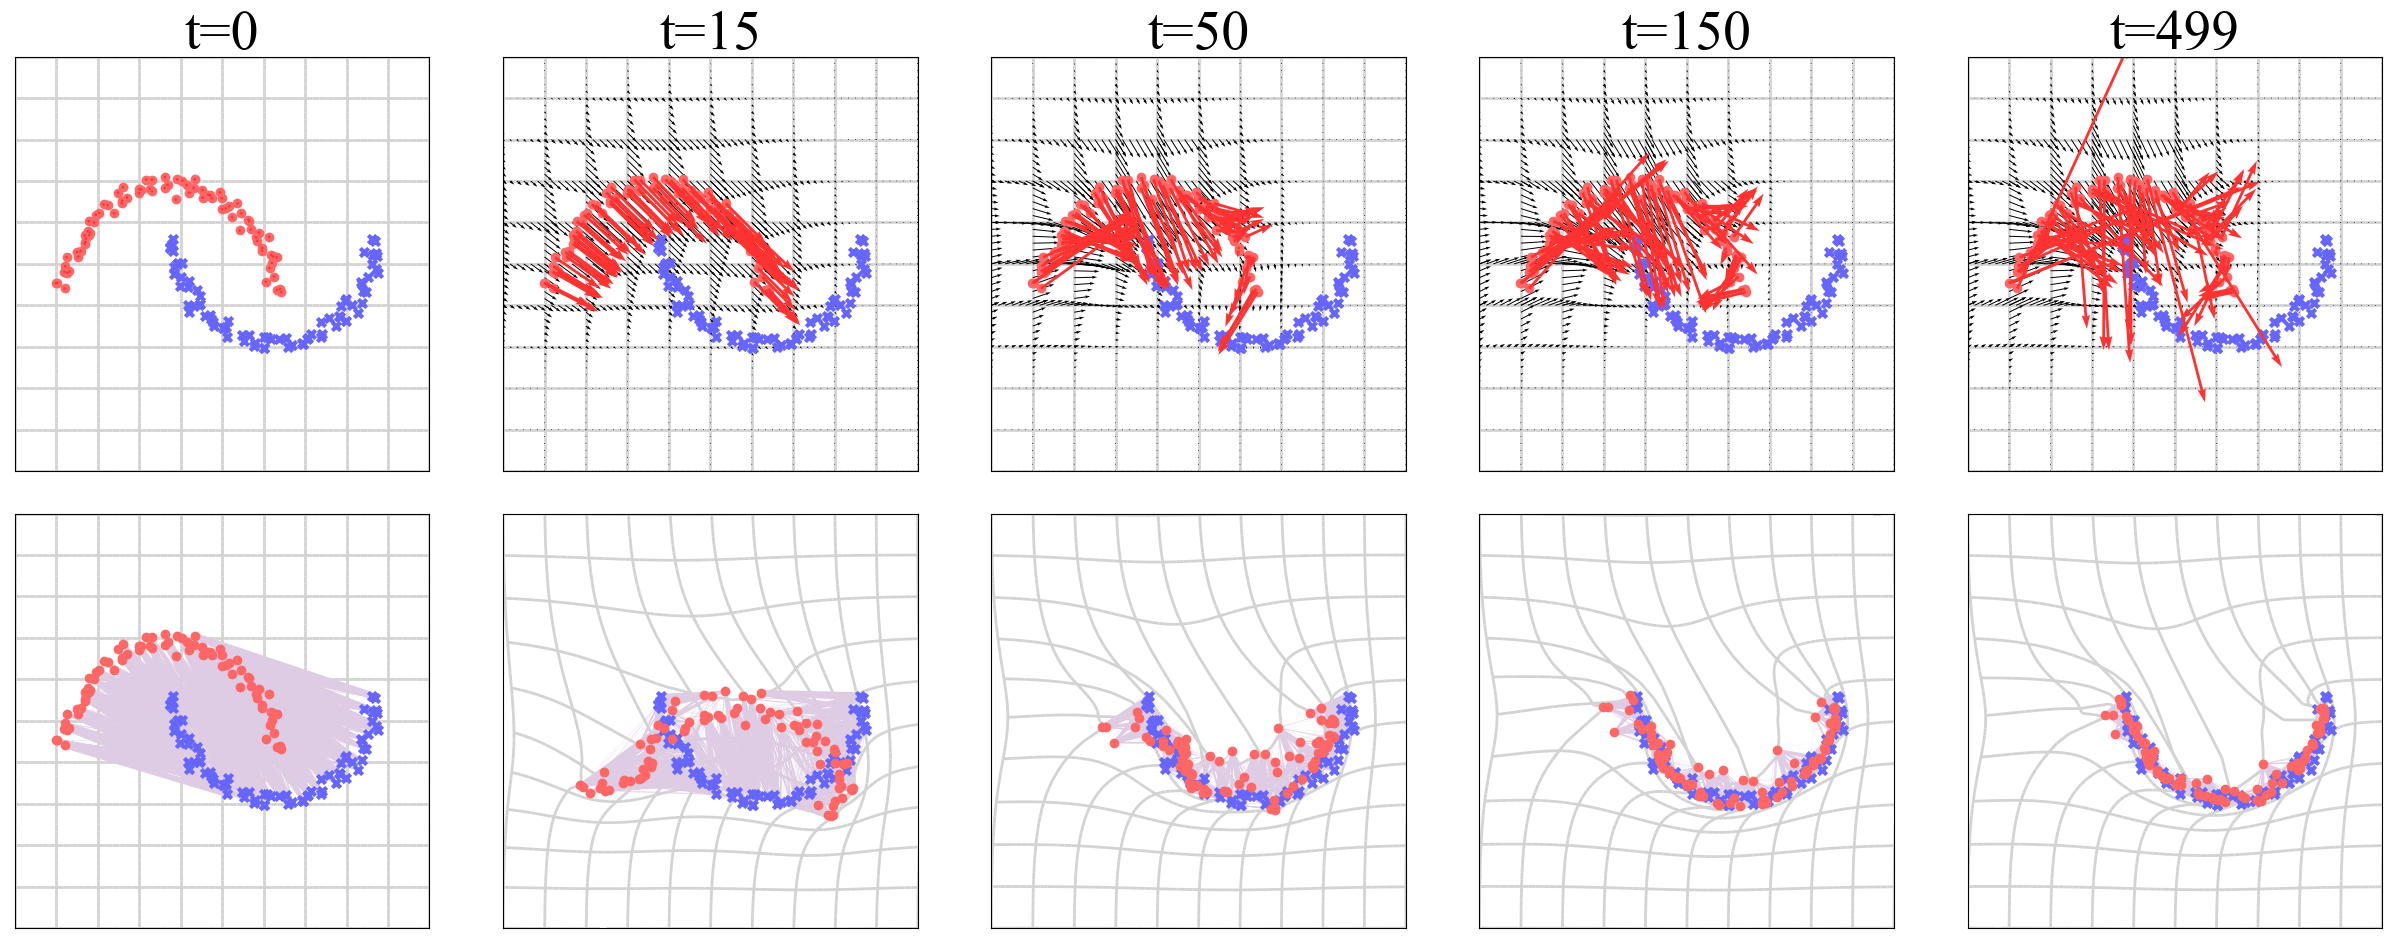
\includegraphics[width=\textwidth]{assets/plt_lddmm_points_moons_training}
%     \caption{Training dynamics of usage of optimal transport cost for registering points}
%     \label{fig:plt_lddmm_points_training}
% \end{figure}
% \end{center} 


 
% \begin{center} 
% \begin{figure}[h!]
%     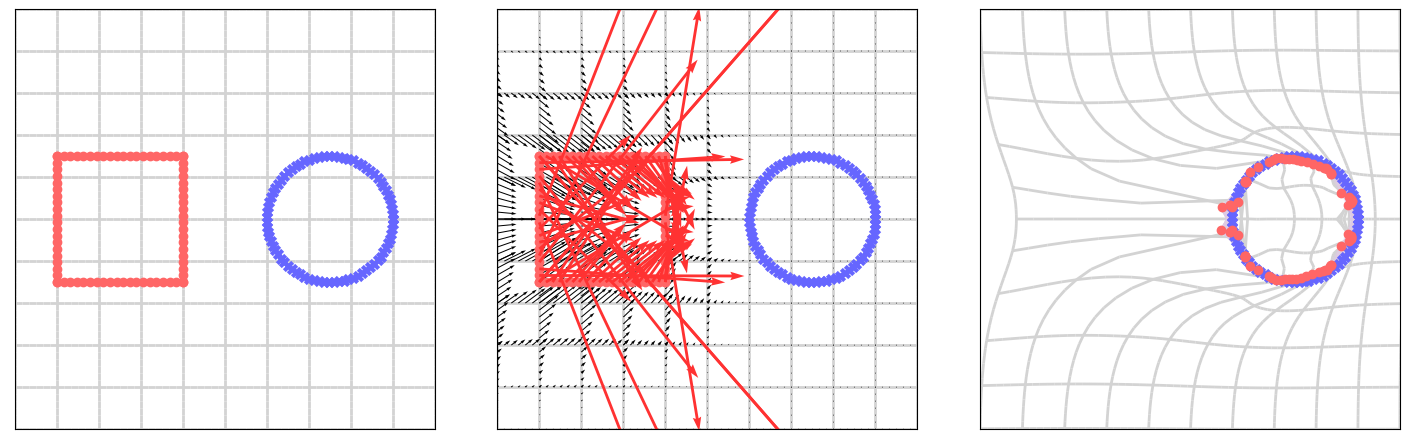
\includegraphics[width=\textwidth]{assets/plt_lddmm_points_shapes} 
%     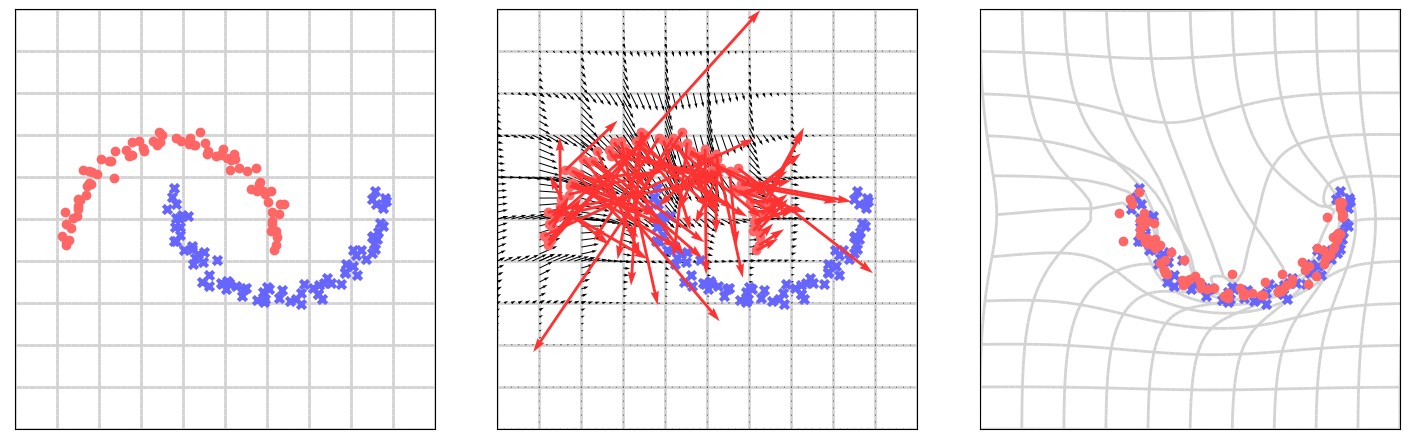
\includegraphics[width=\textwidth]{assets/plt_lddmm_points_moons} 
%     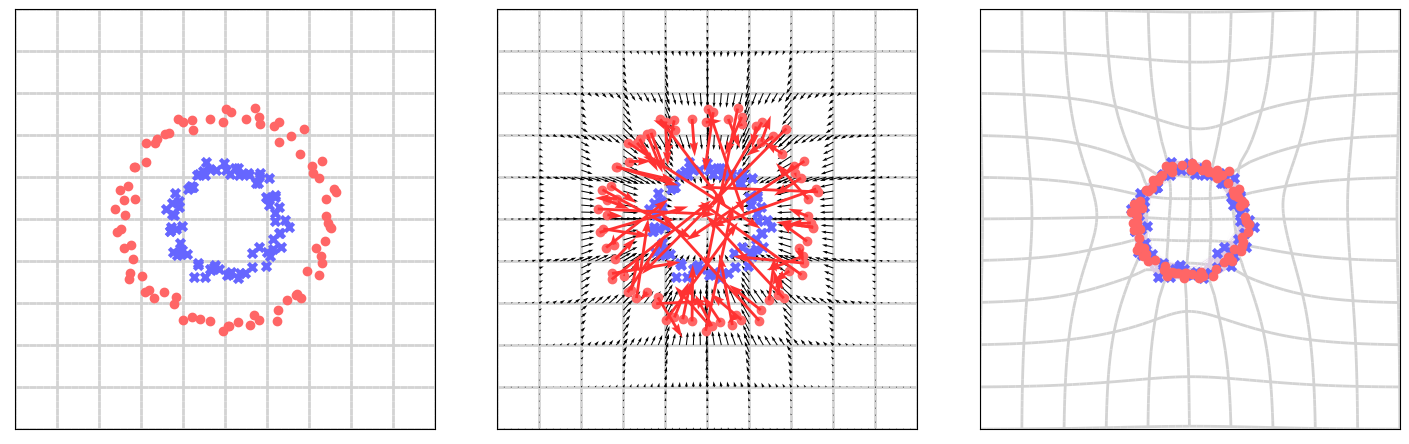
\includegraphics[width=\textwidth]{assets/plt_lddmm_points_circles} 
%     \caption{lddmm with geodesic shooting and entropic regularized unbalanced optimal transport distance as matching loss. Points are encoded as sum of deltas with uniform weights. Shooting's kernel is a sum of radial basis kernel with $\ell \in \pc{.025,.15,.3}$ so as to be able to distinguish points both close and far away. }
%     \label{fig:plt_lddmm_points}
% \end{figure}
% \end{center} 
    
  






% \section{Monge's and Kantorovich's formulation}

% Given $a,b \in \triangle^{n-1}$, where $\triangle^{n-1}$ is unit simplex. $\alpha = \sum_{i=1}^n a_i \delta_{x_i}, \beta = \sum_{j=1}^m b_j \delta_{y_i}$ are discrete measures. The optimal transport problem tries to find a map that associate each point $x_i$ to a single point $y_j$ such that masses are preserved. This corresponds to classical Monge's formulation of optimal transport
% \begin{align}
%     \min_{T:\sX\to\sY: T_{\#}\alpha = \beta}\,
%         &\sum_{i=1}^n c(x_i, T(x_i))
% \end{align}



% where $c:\sX\times\sY \to\R$ is cost defined over support of measures, and that the constraints is simply that $T$ is constrained to be a pushforward from $\alpha$ to $\beta$. The problem with Monge's formulation is that the problem is combinatorial and nonconvex, so hard to solve. Kantorovich relax the deterministic nature of transport map, allowing mass at each source point split and be dispatched to multiple target points. This information is encoded in $P\in\R^{n\times m}_+$, where $P_{ij}$ describes amount of mass flowing from $x_i$ to $y_j$. The Kantorovich formulation of optimal transport for discrete measures is then
% \begin{align}
%     \min_{P\in\R^{n\times m}_+: P1_m = a,\, P^T1_n = b}\,
%         &\inner{C}{P}
% \end{align}
% where the constraints specifies the set of admissible transport map to be a coupling of marginals $\alpha,\beta$ and $C\in\R^{n\times m}$ is the cost matrix, i.e. $C_{ij} = c(x_i,y_j)$. The optimization problem is a linear program and hence can be easily solved using simplex algorithm. In addition, we can instead solve the dual problem, and because of zero duality gap, equivalently solves the primal problem,
% \begin{align}
%     \max_{f,g\in\R^n\times\R^m: f_i+g_j \leq C_{ij}}\,
%         &\inner{f}{a} + \inner{g}{b} 
% \end{align}
% where $f,g$ are called dual potential.

% \section{Entropic Regularization}

% Regularizing the original optimal transport problem brings computational and statistical benefits. In particular, the optimization problem can now be solved with fast matrix scaling algorithms that scales with strength of regularization. In addition, the sample efficiency for regularized problem is also superior. The entropy and KL divergence of coupling between two discrete measure is given by
% \begin{align}
%     H(P)
%         &= -\sum_{i,j} P_{ij}(\log(P_{ij})-1)
%         = - \inner{P}{\log P} + 1^TP1 \\
%     \text{KL}(P\Vert K)
%         &= \sum_{i,j} P_{ij} \log \frac{P_{ij}}{K_{ij}} - P_{ij} + K_{ij}
%         = \inner{P}{\log(P\oslash K)} + 1^T(K-P)1
% \end{align}
% where taking logarithm and subtraction are elementwise operations. The entropic regularized problem
% \begin{align}
%     \min_{P\in\R^{n\times m}_+:P1_m=a,P^T1_n=b}\,
%         &\inner{P}{C} - \epsilon H(P)
%     \label{eq:opt_entropic_regularized_ot}
% \end{align}
% We can interpret primal objective as the information projection of the Gibbs kernel $K\in\R^{n\times m}$ where $K_{ij}=e^{-\frac{C_{ij}}{\epsilon}}$ onto the admissible couplings $U(a,b)=\pc{P\in\R^{n\times m}_+\mid P1_m=a,\, P^T1_n=b}$.
% \begin{align}
%     \inner{P}{C} + \epsilon\inner{P}{\log P} - \epsilon 1^T P 1
%         = \epsilon \inner{P}{\log\left(P \oslash e^{-C/\epsilon} \right)} - \epsilon 1^TP1 + \epsilon 1^Te^{-C/\epsilon}1
%         = \epsilon \text{KL}(P\Vert K)
% \end{align}

% \subsection{Sinkhorn's Algorithm}

% We can solve regularized optimal transport problem with Sinkhorn algorithm \cite{cuturiSinkhornDistancesLightspeed2013}. The basic idea is to write the 1st order optimality condition for the primal variables for the Lagrangian,
% \begin{align}
%     \sL(P,f,g)
%         &= \inner{P}{C} - \epsilon H(P) - \inner{f}{P1_m-a}- \inner{g}{P^T1_n-b} \\
%     \partial \sL(P,f,g)/\partial P_{ij}
%         &= C_{ij} + \epsilon \log(P_{ij}) - f_i - g_j = 0
%         \quad\Rightarrow\quad
%         P_{ij} = e^{(-C_{ij}+f_i+g_j)/\epsilon}
% \end{align}

% % Note optimal $P$ can be written as scaling of Gibbs kernel row-wise by $u=e^{f/\epsilon}$ and column-wise by $v=e^{g/\epsilon}$, i.e. $P=\diag(u)K \diag(v)$. Substitute expression for $P$ into marginal constraints, get $a = \diag(u) K \diag(v) 1_m = u\odot (Kv)$ and $b = v\odot (K^T u)$. The Sinkhorn's algorithm updates $u,v$ alternatingly
% \begin{align}
%     u^{(\ell+1)} 
%         \leftarrow a \oslash (Kv^{(\ell)}) 
%     \quad\quad
%     v^{(\ell+1)}
%         \leftarrow b \oslash (K^Tu^{(\ell+1)})
% \end{align}
% Each iteration of the algorithm uses $\sO(nm)$ computation for matrix-vector products and can be accelerated to $\sO(n\log n)$ using convolution if suppport is over gridded space. 
% \subsection{Log-domain Stabilization}

% Sinkhorn's iteration can be numerically unstable as $\epsilon\to 0$ due zeros in $K$, resulting in null values during division by zero. One solution is to perform computation of $u,v$ in the log-domain \cite{chizatScalingAlgorithmsUnbalanced2017, schmitzerStabilizedSparseScaling2019}. This is equivalent to block coordinate ascent on the dual of entropic regularized optimal transport problem (\ref{eq:opt_entropic_regularized_ot}),
% \begin{align}
%     \max_{f,g\in\R^{n\times m}} \inner{f}{a} + \inner{g}{b} - \epsilon\inner{e^{f/\epsilon}}{Ke^{g/\epsilon}}
% \end{align}
% Then $0 = \partial L_{\text{dual}}(f,g)/\partial f = a - e^{f/\epsilon} \odot (Ke^{g/\epsilon})$ implies $f = \epsilon \log(a) - \epsilon \log(Ke^{g/\epsilon})$ and similarly for $g$. So,
% \begin{align}
%     f^{(\ell+1)}
%         \leftarrow \epsilon \log(a) - \epsilon\log(Ke^{g^{(\ell)}/\epsilon})
%     \quad\quad
%     g^{(\ell+1)}
%         \leftarrow \epsilon \log(b) - \epsilon\log(Ke^{f^{(\ell+1)}/\epsilon})
%     \label{eq:sinkhorn_dual_ascent}
% \end{align}
% This is equivalent to Sinkhorn's iteration in log domain. Additionally, we can define a numerically stable softmin operator based on log-sum-exp, $\text{softmin}_{\epsilon}(z) = - \epsilon \log \sum_{i} e^{-z_i/\epsilon} = -\epsilon \text{LSE}(-z/\epsilon)$. Note $f_i = \epsilon \log a_i - \epsilon \log \sum_j e^{-(C_{ij}-g_j)/\epsilon} =\text{softmin}_{\epsilon}(C_{ij}-f_i-g_j) + f_i +  \epsilon \log a_i$. Therefore, (\ref{eq:sinkhorn_dual_ascent}) can be equivalently written as,
% \begin{align}
%     f^{(\ell+1)}
%         &\leftarrow \text{softmin}_{\epsilon} (S(f^{(\ell)}, g^{(\ell)})) + f^{(\ell)} + \epsilon \log(a) \\ 
%     g^{(\ell+1)}
%         &\leftarrow \text{softmin}_{\epsilon} (S(f^{(\ell+1)}, g^{(\ell)})) + g^{(\ell)} + \epsilon \log(b)
%     \label{eq:sinkhorn_dual_ascent2}
% \end{align}
% where $S(f,g)_{ij} = C_{ij}-f_i-g_j$. 


% \subsection{Minimum Kantorovich Estimator}

 

% \section{Unbalanced Transport}

% Previously, optimal transprot problem requires $\alpha,\beta$ to have equal mass. This becomes a problem in applications when either the measures are noisy or when preservation of mass is not desirable. We can relax hard marginal constraints with soft penalty that measures deviation from exact coupling using some divergence, e.g. KL-divergence \cite{chizatScalingAlgorithmsUnbalanced2017},
% \begin{align}
%     \min_{P\in\R^{n\times m}_+}\, 
%         \inner{P}{C} - \epsilon H(P) + \rho \text{KL}(P1_m \Vert a) + \rho \text{KL}(P^T 1_m \Vert b)
% \end{align}
% Similar to balanced case, we can show that optimal coupling is again a scaling of $K$, i.e. $P = \diag(u) K \diag(v)$ where $u = (a \oslash (Kv))^{\lambda}$ and $v = (b \oslash (K^T u))^{\lambda}$ where $\lambda = \frac{\rho}{\rho + \epsilon}$ \cite{frognerLearningWassersteinLoss2015}. We can derive a similar Sinkhorn iteration in the log domain for unbalanced case.







% \begin{figure}[t]
% \centering
%  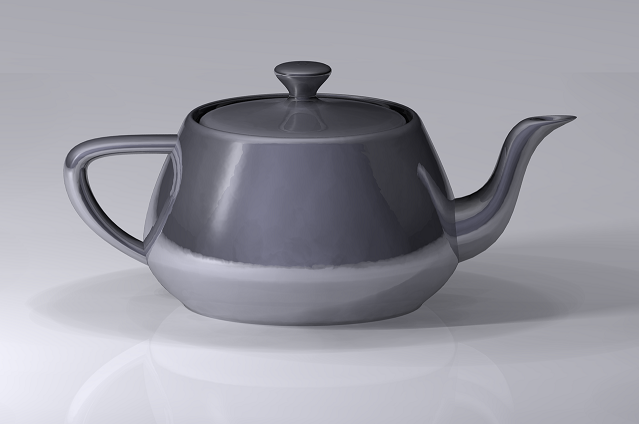
\includegraphics[width=.75\linewidth]{teapot}
% \caption{This is an example of a single-column figure.}\label{fig:teapot}
% \end{figure}

% A description in words, equations, algorithm listings, and/or flow charts describing your approach.  

% Some useful \LaTeX\ tips:  Inline equations are useful for small expressions, like $E=mc^2$.  Unnumbered equations can take up more space:
% $$\int_\Omega \nabla\cdot F\,dV= \oint_{\partial\Omega} F\cdot\hat n\,dA.$$
% If you need a number in an equation, you can do that as follows:
% \begin{align}\label{eq:green}
%     \int_U (\varphi\Delta\psi + \nabla\varphi\cdot\nabla\varphi)\,dV=\oint_{\partial U}\psi(\nabla\varphi\cdot\hat n)\,dA. \\
%     sfds &= sdfs
% \end{align}
% Then you can refer to equation numbers like~\eqref{eq:green}.  If you use \texttt{label}, you can refer to other items, like sections \S\ref{sec:technical_approach} and figures, e.g.\ Figure~\ref{fig:teapot}.  Never hard-code the number of a section, equation, or figure!

\section{Results}

Figures/tables illustrating the results of your work, as well as text interpreting these results. \cite{peyreComputationalOptimalTransport2020},


\bibliographystyle{eg-alpha-doi}
\bibliography{optimal_transport,registration,GP}


\end{document}
